\documentclass[dvipdfmx, border={2pt 2pt 2pt 2pt}]{standalone}

\usepackage{amssymb}
\usepackage{tikz}
\usetikzlibrary{arrows, automata, positioning, shapes}
\usetikzlibrary{arrows.meta}

\begin{document}	\centering
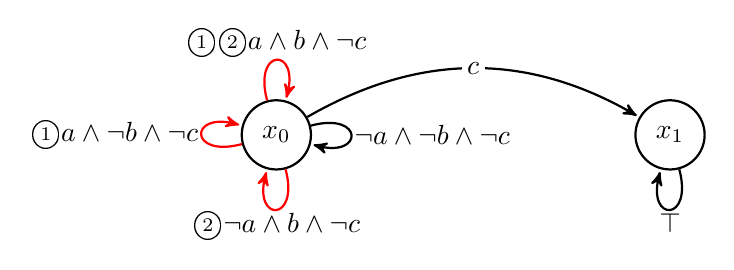
\begin{tikzpicture}[
	->,
	>=stealth',
	shorten >=1pt,
%	auto,
	node distance=5cm,
	initial text=, 
	thick
]

%\tikzset{every edge/.append style={
%		sloped
%%		font=\tiny  %\scriptsize \tiny
%}}
\node[state] (x0) [ellipse]                   {$x_0$};
\node[state] (x1) [ellipse,right of=x0] {$x_1$};
%\node[state] (x2) [ellipse,right=4.5cm] at (x1) {$(x_0,(1,0)^T)$};
%\node[state] (x3) [ellipse,right=4.5cm] at (x0) {$(x_1,(*,*)^T)$};

{
\tikzstyle{every node}=[inner sep = 1pt,fill=none,black]
\tikzset{every loop/.style={min distance=7mm,looseness=5}}
\path 	(x0)edge [bend left=30,align=center] node [inner sep=2pt,fill=white] {$ c $} (x1)
			edge [loop above,red] node [fill=none] {\textcircled{\scriptsize 1}\textcircled{\scriptsize 2}$ a \land b \land \neg c $} (x0)
			edge [loop left,red] node {\textcircled{\scriptsize 1}$ a \land \neg b \land \neg c $} (x0)
			edge [loop below,red] node {\textcircled{\scriptsize 2}$ \neg a \land b \land \neg c $} (x0)
			edge [loop right] node {$ \neg a \land \neg b \land \neg c $} (x0)
		(x1)edge [loop below] node [fill=none] {$ \top $} (x1)
%			edge [loop left,red] node  {} (x1)
%			edge [bend left=45,red] node  {} (x0)
%			edge [bend left=25,red] node  {\textcircled{\scriptsize 1}$ a \land \neg b \land \neg c $} (x2)
;
}
%\tikzstyle{every node}=[inner sep = 1pt,fill=white,black]
%\node[draw=none,fill=white] (e01) [below=2.3cm] at (x0) {$ a \land b \land \neg c $};
%\node[draw=none,fill=white] (e01.acc) [fill=none,above=0.15cm] at (e01) {\textcircled{\scriptsize 1}\textcircled{\scriptsize 2}};
%\node[draw=none,fill=white] (e02) [above right=0.75cm] at (e01) {\textcircled{\scriptsize 1}$ a \land \neg b \land \neg c $};
%%\node[draw=none,fill=white,align=center] (e02.acc) [fill=none,above=0.15cm] at (e02) {\textcircled{\scriptsize 1}};
%\node[draw=none,fill=white] (e02) [left=1.5cm] at (x0) {$ \neg a \land \neg b \land \neg c $};
%\node[draw=none,fill=white] (e11) [above left=0.75cm] at (e01) {\textcircled{\scriptsize 2}$ \neg a \land b \land \neg c $};
%\node[draw=none,fill=white] (e12) [left=1.5cm] at (x1) {$ \neg a \land \neg b \land \neg c $};
%\node[draw=none,fill=white,align=center] (e12.acc) [fill=none,above=0.15cm] at (e12) {\textcircled{\scriptsize 1}\textcircled{\scriptsize 2}};
%\node[draw=none,fill=white] (e20) [right=1.5cm] at (x2) {$ \neg a \land \neg b \land \neg c $};
\end{tikzpicture}
\end{document}